%% Epilogue — The Boring Service
\frontchapter{The Boring Service}{Epilogue}
\chaptersubtitle{Fifteen weeks, one chat model, and the quiet triumph of nothing happening}

\begin{calloutbox}{tbbblue}{tbbbluefill}
{\normalsize\bfseries\color{tbbblue}What this is (and is not)}\par\vspace{3pt}
This epilogue has no learning objectives, no lab, no exercises, and nothing on the exam. It is meant to be read the way you would walk through a museum of a trip you actually took: after the demo, with coffee, at whatever pace amuses you. Inside: a \textbf{biography} of the service you built, a \textbf{souvenir cabinet} of the one-liners you earned, a \textbf{dinner party} you are now qualified to attend, a \textbf{warranty card} stating which parts of this book expire and which are guaranteed for ten years, and a short \textbf{letter} for a night that has not happened to you yet — but will.
\end{calloutbox}

\vspace{4.0pt}

\namedsection{E.1}{The Biography of a Service}

It was born in Week 1 as an embarrassment: \textbf{thirty seconds of silence and a spinning cursor}, wrapped around 0.31 seconds of flawless model execution. Exhibit A was never really about the bug (a cold model loading on the first request, a queue nobody had drawn). It was about the diagnosis that took a whole course to learn to make in two lines — \textit{which segment is the bottleneck?} — and about the announcement hiding inside it: a trained model and a working service are different artifacts, separated by everything this book turned out to be. The service spent its first week as most services do — a perfect brain with no body, no manners, no promises, and no idea what anything costs.

Weeks 2 through 5 were body-building. It got a \textbf{machine}, and immediately learned the machine was a polite fiction — a guest on a hypervisor, its GPU real only because passthrough hands the silicon through the fiction untouched (the one part of the rental that is not virtualized is the part you pay for). It got \textbf{cages and meters} — namespaces so it could only see itself, cgroups so it could only eat its share — and it died for the first time: \code{exit 137}, the kernel's goodbye note, which is also the only arithmetic this book asks you to memorize forever (128 + signal 9). It got a \textbf{shippable body}: an image, layered and digest-pinned, so that "works on my machine" became "IS my machine, byte for byte, anywhere." And it got \textbf{reflexes}: probes that gate traffic and restarts that need no meeting, a fleet manager that treats your intentions as a database and reality as a bug to be fixed. By Week 5 it could survive its own death. It still could not be \textit{trusted} — reflexes act; they do not explain. That debt would sit quietly until Week 14.

Week 6 gave it a \textbf{door} — a load balancer, TLS, a key, a quota — and with the door came the course's first genuinely commercial sentence: the difference between \textit{a container that answers curl} and \textit{a service someone could be billed for} is the door. The door also introduced the outside world's many vocabularies of refusal (503, 504, the stream that dies mid-sentence), and the discipline of standing outside your own walls to check them — a habit that looked like paranoia in Week 6 and became a paging policy in Week 14.

Week 7 was adolescence: the service learned to \textbf{make a promise}. Not "be fast" — a promise with a shape: \textit{p99 ≤ 500 ms, measured here, over this window, at this load, under this budget}. It learned percentile grammar (the mean describes nobody; percentiles neither add nor average — a rule that returned twice more, wearing histograms). It got an allowance — the error budget — which converted reliability from a virtue contest into a ledger. And then the first bill arrived: \textbf{\$4,762 a month} for the naive fleet, a number that hung over the course like a parent's eyebrow for five straight weeks. Week 9 sent crowds at it (and taught it that most storms are self-inflicted: the retry storm remains the only weather system in this book that the victims personally organize), and taught it to say no early and cheaply — \textit{the refusal is the product}. Week 10 put it on a diet with a ceremony: INT8 at half the cost, admitted only through a gate whose tolerance was written down \textit{before} the measurement — because lossy without a gate is just hoping, at scale. Bill: \textbf{\$2,381}.

Week 11 is when it \textbf{learned to talk}, and talking changed its physics. One latency became two clocks (the wait for the first word; the pace of every word after). Memory became real estate: 112 KB per token of KV cache, 448 MiB for one long conversation, seats at the table priced by the megabyte and filled by continuous batching — and the great allocator's trick, PagedAttention, which took malloc's oldest tragedy (reserve for the maximum, waste the difference) and fixed it the way operating systems fixed it in 1962: a page table. The SLO was re-negotiated for streams, in public, with arithmetic. Week 12 taught it to \textbf{breathe} — replicas that follow the day's staircase (pods chase waves; nodes follow forecasts), cold starts priced honestly at 150 seconds, capacity bought the way Samuel Insull sold electricity: a committed floor for the base, spot for the peaks, and useful work found for the valleys. Bill: \textbf{\$1,513}, then \textbf{\$877} — and the course's quietest lesson: \textit{build-vs-buy was never a slogan; it was a load factor}.

Week 13 taught it to \textbf{change without drama}. The Friday deploy — a perfect model wrecked by a config file traveling alone — begat the registry (a release is a \textit{triple} of digests with its evidence stapled on), the pipeline (whose red runs are the product: Fridays that didn't happen), and the canary (Haldane's bird, reborn with an automated retreat reflex). The deploy became the most boring sentence in engineering: \textit{automated, versioned, gradual, reversible}. And Week 14 completed the nervous system with the three things reflexes never had: \textbf{memory} (four dashboard rows, ordered exactly as a 2 a.m. brain asks its questions), \textbf{attention} (pages that fire on burn rates rather than vibes — and rarely, because alarm fatigue has a body count), and \textbf{foresight} (drift watched weekly, because canaries catch cliffs and the world prefers slopes). Its first real incident — a neighbor on its GPU, the very mystery Week 12 had promised — lasted twenty minutes and produced three action items and zero blame. The bill closed at \textbf{\$900, exactly}: the last \$23 being the part that watches all the other parts.

And in Week 15 it stood in front of strangers and was demonstrated. If everything went as designed, the demo was — say it with pride — \textbf{boring}. Traffic through a door with a key, answers inside a promise with a number, a bill that ends in a chosen figure, a dashboard breathing gently in the corner of the projector. Boring, in operations, is not the absence of excitement; it is excitement \textit{paid off in advance}, in gates and rehearsals and graphs drawn at 2 p.m. The service's biography ends the way all good infrastructure biographies end: with nothing happening, on purpose, in public.

\begin{tbbfigure}
  \adjustbox{max width=0.94\linewidth,max totalheight=0.46\textheight}{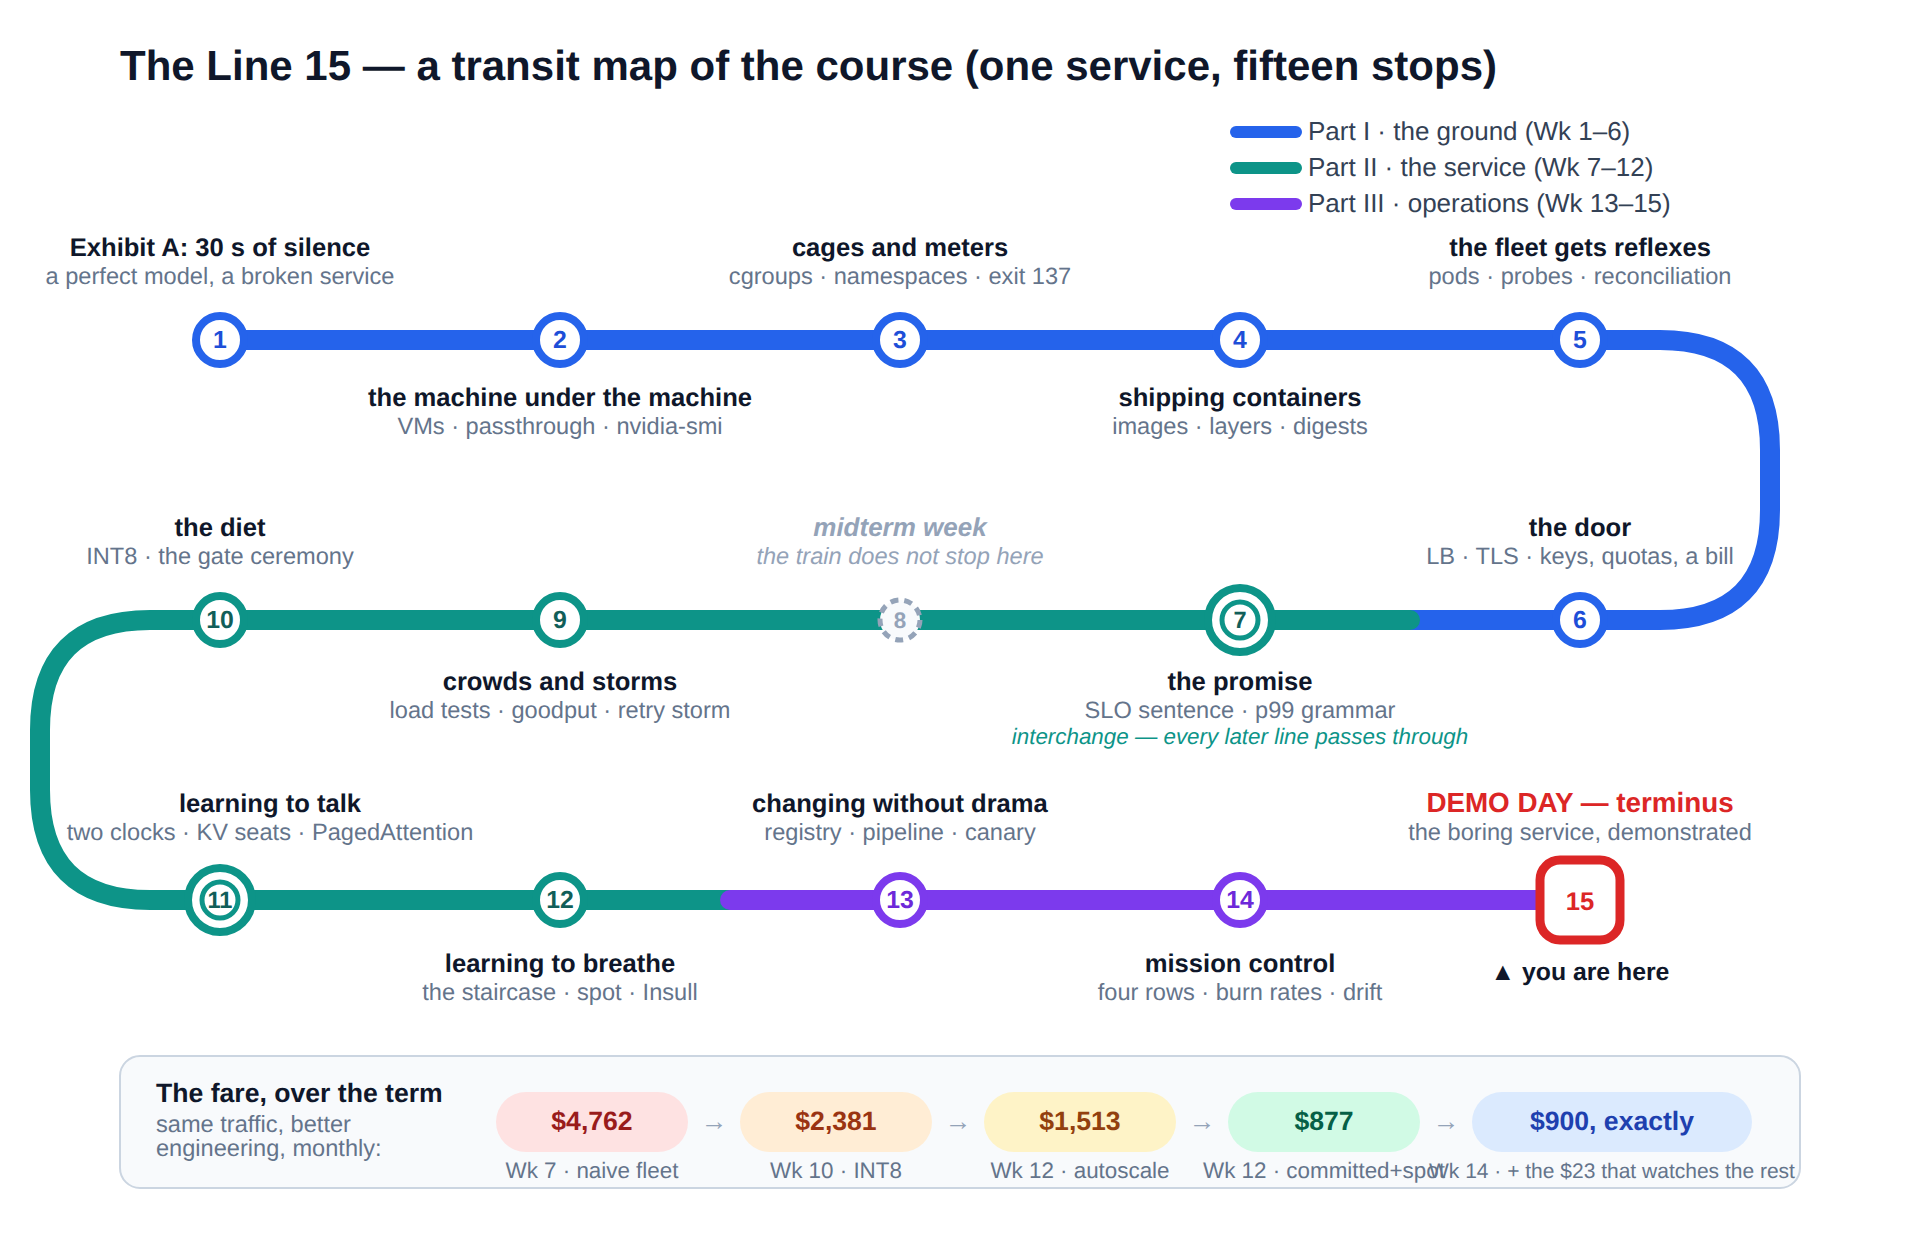
\includegraphics{figures/figE-1_line15.png}}\\[3pt]
  \figcaption{Figure E-1  The Line 15. One service, fifteen stops, three fare zones — and the fare falling from \$4,762 to a chosen \$900 as the engineering improved. The train does not stop at Week 8. Terminus: the boring service, demonstrated. You are here.}
\end{tbbfigure}

\namedsection{E.2}{The Souvenir Cabinet}

Every chapter of this book planted at least one deliberately portable sentence — short enough to survive in a tired brain, sharp enough to make a decision with. This was not a stylistic tic; it was the point. Production engineering is mostly performed by people at their cognitive worst (2 a.m., demo day, week nine of a quarter), and a good aphorism is \textbf{compression for degraded hardware}: the whole argument, pre-computed, cached where the sleep-deprived can still reach it. Here they are, on museum plaques, with the incident that earned each one. Dust them occasionally.

\begin{tbbtablewrap}
  \begin{tabular}{@{}>{\raggedright\arraybackslash}m{\dimexpr 0.3564\tbltextwidth-2\tabcolsep\relax} >{\raggedright\arraybackslash}m{\dimexpr 0.1596\tbltextwidth-2\tabcolsep\relax} >{\raggedright\arraybackslash}m{\dimexpr 0.4840\tbltextwidth-2\tabcolsep\relax}@{}}
  \arrayrulecolor{tbbnavy}\specialrule{1pt}{0pt}{0pt}
  \rowcolor{tbbtablehead}{\centering \bfseries\color{tbbnavy}Souvenir} & {\centering \bfseries\color{tbbnavy}Earned} & {\centering \bfseries\color{tbbnavy}Why it keeps} \\
  \arrayrulecolor{tbbnavy}\specialrule{0.7pt}{0pt}{2pt}
  {\textbf{exit 137 — the kernel's goodbye note}} & {Wk 3} & {Every OOM you will ever meet, in any orchestrator, forever: 128 + 9. The limit was real and the meter was honest.} \\
  \arrayrulecolor{tbbtableborder}\hline
  {\textbf{Your view of a system is only as honest as your mounts}} & {Wk 3} & {From ps in a namespace to exporters reading cgroup files: instrumentation lies unless you check what it reads.} \\
  \arrayrulecolor{tbbtableborder}\hline
  {\textbf{Tags drift; digests can't}} & {Wk 4} & {The whole Week-13 registry was this sentence, grown up. Version by content, not by label, and rollback becomes a pointer.} \\
  \arrayrulecolor{tbbtableborder}\hline
  {\textbf{Probes are reflexes; monitoring is memory}} & {Wk 5 → 14} & {Self-healing without observability is incident suppression. You need both nervous systems; they are not rivals.} \\
  \arrayrulecolor{tbbtableborder}\hline
  {\textbf{One health endpoint is the single source of truth}} & {Wk 6} & {Two definitions of "healthy" will disagree during exactly one incident per quarter, always the worst one.} \\
  \arrayrulecolor{tbbtableborder}\hline
  {\textbf{The mean describes nobody}} & {Wk 7} & {The single most repeated sentence in the book, because it is the single most repeated mistake in the field.} \\
  \arrayrulecolor{tbbtableborder}\hline
  {\textbf{Percentiles don't add, and never average}} & {Wk 7 → 14} & {Why serious systems ship histograms. avg-of-p99s once said 2.76 s where the truth was 9.08.} \\
  \arrayrulecolor{tbbtableborder}\hline
  {\textbf{L = λW}} & {Wk 7 → 11} & {The only formula that follows you into meetings: seats, arrival rates, and wait times, one algebra for queues and KV pools alike.} \\
  \arrayrulecolor{tbbtableborder}\hline
  {\textbf{A fast no beats a slow maybe (the refusal is the product)}} & {Wk 9} & {Shed early, shed cheaply. Every system that queues into futility feeds its own storm.} \\
  \arrayrulecolor{tbbtableborder}\hline
  {\textbf{The tolerance predates the number}} & {Wk 10} & {Decide what "good enough" means before you measure, or the measurement will decide for you. Lossy needs a ceremony.} \\
  \arrayrulecolor{tbbtableborder}\hline
  {\textbf{Pinned-high is healthy; the alarm lives in the queue}} & {Wk 11} & {A full cache is the design working; a growing queue is demand outrunning seats. Misreading this gauge is a rite of passage — skip it.} \\
  \arrayrulecolor{tbbtableborder}\hline
  {\textbf{Pods chase waves; nodes follow forecasts}} & {Wk 12} & {Two timescales, two mechanisms, one bill. Autoscaling in six words.} \\
  \arrayrulecolor{tbbtableborder}\hline
  {\textbf{Boring = automated + versioned + gradual + reversible (+ observed)}} & {Wk 13 → 14} & {The deploy sentence, with Week 14's amendment. Boring is the highest compliment operations can pay.} \\
  \arrayrulecolor{tbbtableborder}\hline
  {\textbf{Canaries catch cliffs, not slopes}} & {Wk 13} & {Every instrument has a blind timescale. Pair the minutes-instrument with a weeks-instrument or the world will drift past both.} \\
  \arrayrulecolor{tbbtableborder}\hline
  {\textbf{Page on symptoms; ticket on causes}} & {Wk 14} & {The two-word routing rule that keeps rotations sane and pagers trusted. Hospitals paid the tuition for this one.} \\
  \arrayrulecolor{tbbtableborder}\hline
  {\textbf{At 2 a.m. you can only see what you graphed at 2 p.m.}} & {Wk 14} & {The chapter-in-one-sentence of the whole operational half of this book. Draw the questions before the night asks them.} \\
  \arrayrulecolor{tbbnavy}\specialrule{1pt}{2pt}{0pt}
  \end{tabular}\par
  \figcaption{The souvenir cabinet. Sixteen plaques, fifteen weeks. If you keep only one: the last one — it contains instructions for keeping the rest.}
\end{tbbtablewrap}

\namedsection{E.3}{The Dinner Party}

This book had a nervous habit: whenever the going got genuinely hard, it left the room — not for another chapter, for another \textit{century}. The bill arrived in Week 7 and the course fled to \textbf{1902}, to a man selling kilowatt-hours to streetcars and ice houses. The fleet needed sizing and it fled to \textbf{1961}, to a proof about queues that assumed nothing and therefore survives everything. The KV pool shattered into unusable fragments and it fled to \textbf{1962}, to the page table. The deploy needed a verdict and it fled to the \textbf{1890s}, to a physiologist carrying warm-blooded sentinels into coal mines; the pager needed manners and it fled to \textbf{1969}, to a room in Houston reading four-digit alarm codes off a hand-written sheet. This was never decoration. It was the course's deepest claim, made by repetition until you stopped noticing it: \textbf{the hard problems of serving are not new problems.} They are old problems that changed units — kilowatts into GPU-hours, trunk lines into seats, carbon monoxide into bad percentiles — and the people who solved them first are, professionally speaking, your colleagues now.

Hence the dinner party: the epilogue's only examination, and it is self-administered. Could you hold your seat at a table of people who died before your stack was invented? Fifteen weeks ago the honest answer was no — not for lack of intelligence, but for lack of \textit{shared bills}. You had never paid for idle capacity, never signed a percentile, never bet a fleet on a sentinel, never been woken by a machine that was right to wake you. Now you have. You are qualified for this table not because you learned these people's fields but because you have been invoiced by the same universe: peaks and valleys, seats and waits, cliffs and slopes, the crew and the bird. The seating is arranged accordingly — each chair numbered by \textbf{the week that mailed the invitation}.

\begin{tbbtablewrap}
  \begin{tabular}{@{}>{\raggedright\arraybackslash}m{\dimexpr 0.0957\tbltextwidth-2\tabcolsep\relax} >{\raggedright\arraybackslash}m{\dimexpr 0.2074\tbltextwidth-2\tabcolsep\relax} >{\raggedright\arraybackslash}m{\dimexpr 0.3138\tbltextwidth-2\tabcolsep\relax} >{\raggedright\arraybackslash}m{\dimexpr 0.3830\tbltextwidth-2\tabcolsep\relax}@{}}
  \arrayrulecolor{tbbnavy}\specialrule{1pt}{0pt}{0pt}
  \rowcolor{tbbtablehead}{\centering \bfseries\color{tbbnavy}Chair} & {\centering \bfseries\color{tbbnavy}Guest} & {\centering \bfseries\color{tbbnavy}Their version of your problem} & {\centering \bfseries\color{tbbnavy}Table talk} \\
  \arrayrulecolor{tbbnavy}\specialrule{0.7pt}{0pt}{2pt}
  {\centering \textcolor{tbbteal}{\textbf{7}}} & {\textbf{John Little}\newline \textit{queueing, 1961}} & {How many customers are \textit{in} the shop, given how fast they arrive and how long they stay — proved with no assumptions about either.} & {Sketch the KV pool on a napkin and watch him recognize it at once: seats, arrivals, waits. You used his algebra twice — Week 7 for replicas, Week 11 for a cache — and he will note, gently, that it was the same use.} \\
  \arrayrulecolor{tbbtableborder}\hline
  {\centering \textcolor{tbbteal}{\textbf{9}}} & {\textbf{Margaret Hamilton}\newline \textit{Apollo software, 1969}} & {A 4 KB executive that, overloaded during the descent, shed low-priority work by design — and landed anyway.} & {She will ask what your service drops when the crowd arrives, and whether you chose it in advance. Have Week 9's answer ready: \textit{the refusal is the product.} Hers flew to the Moon; yours returns 429s. Same principle, different altitude.} \\
  \arrayrulecolor{tbbtableborder}\hline
  {\centering \textcolor{tbbteal}{\textbf{11}}} & {\textbf{The Atlas paging crew}\newline \textit{Manchester, 1962}} & {Programs demanded contiguous memory; the machine had scattered fragments. Their fix: fixed-size pages, plus a table that translates.} & {Tell them their trick now runs \textit{inside attention itself} — 16-token blocks, waste under 4\%, throughput ×2–4 — and that nobody improved their idea, only re-aimed it. Expect no surprise. Indirection people are unsurprisable.} \\
  \arrayrulecolor{tbbtableborder}\hline
  {\centering \textcolor{tbbteal}{\textbf{12}}} & {\textbf{Samuel Insull}\newline \textit{Chicago Edison, 1902}} & {A power plant sized for the evening lighting peak, idle twenty hours a day. His obsession: \textbf{load factor} — average demand over peak.} & {He will ask, before the soup arrives, what your GPUs do at 4 a.m. If you can answer \textit{the drift evals ride the idle valley} — Week 14's judge on Week 12's committed floor — he will try to hire you before dessert.} \\
  \arrayrulecolor{tbbtableborder}\hline
  {\centering \textcolor{tbbpurple}{\textbf{13}}} & {\textbf{John Scott Haldane}\newline \textit{mine physiology, 1896}} & {A sentinel with a faster metabolism, exposed ahead of the crew: cheap to watch, cheap to act on, minutes of warning.} & {He will approve of your 5\% traffic split, and note without bitterness that the detector that retired his bird took ninety years to arrive — yours watches automatically and retreats in seconds. Then, leaning in: \textit{canaries catch cliffs. What watches your slopes?}} \\
  \arrayrulecolor{tbbtableborder}\hline
  {\centering \textcolor{tbbpurple}{\textbf{14}}} & {\textbf{John Aaron \& Jack Garman}\newline \textit{mission control, 1969}} & {SCE to AUX, recalled from one strange telemetry signature seen in a drill; 1202, resolved off a cheat sheet hand-written after a \textit{failed} simulation.} & {The two best arguments ever staged for recognized signatures over raw genius at 2 a.m. They will ask where your cheat sheet lives (the runbook), which failure wrote it (the lab you broke on purpose, twice), and who updates it after incidents. Answer honestly. These two can tell.} \\
  \arrayrulecolor{tbbtableborder}\hline
  {\centering \textcolor{tbbred}{\textbf{15}}} & {\textbf{You}\newline \textit{fifteen weeks, one service}} & {A perfect model behind thirty seconds of silence, turned into a boring service with its promise in writing.} & {Mostly listen. When the bill comes, observe that it is split by load factor, that yours ends in a chosen number — \textbf{\$900, exactly} — and that every single person at this table understands precisely why that felt so good.} \\
  \arrayrulecolor{tbbnavy}\specialrule{1pt}{2pt}{0pt}
  \end{tabular}\par
  \figcaption{The guest list, in chair order. The kernel was invited on behalf of Weeks 1–6 and sent regrets — someone has to keep the lights on.}
\end{tbbtablewrap}

\begin{tbbfigure}
  \adjustbox{max width=0.94\linewidth,max totalheight=0.46\textheight}{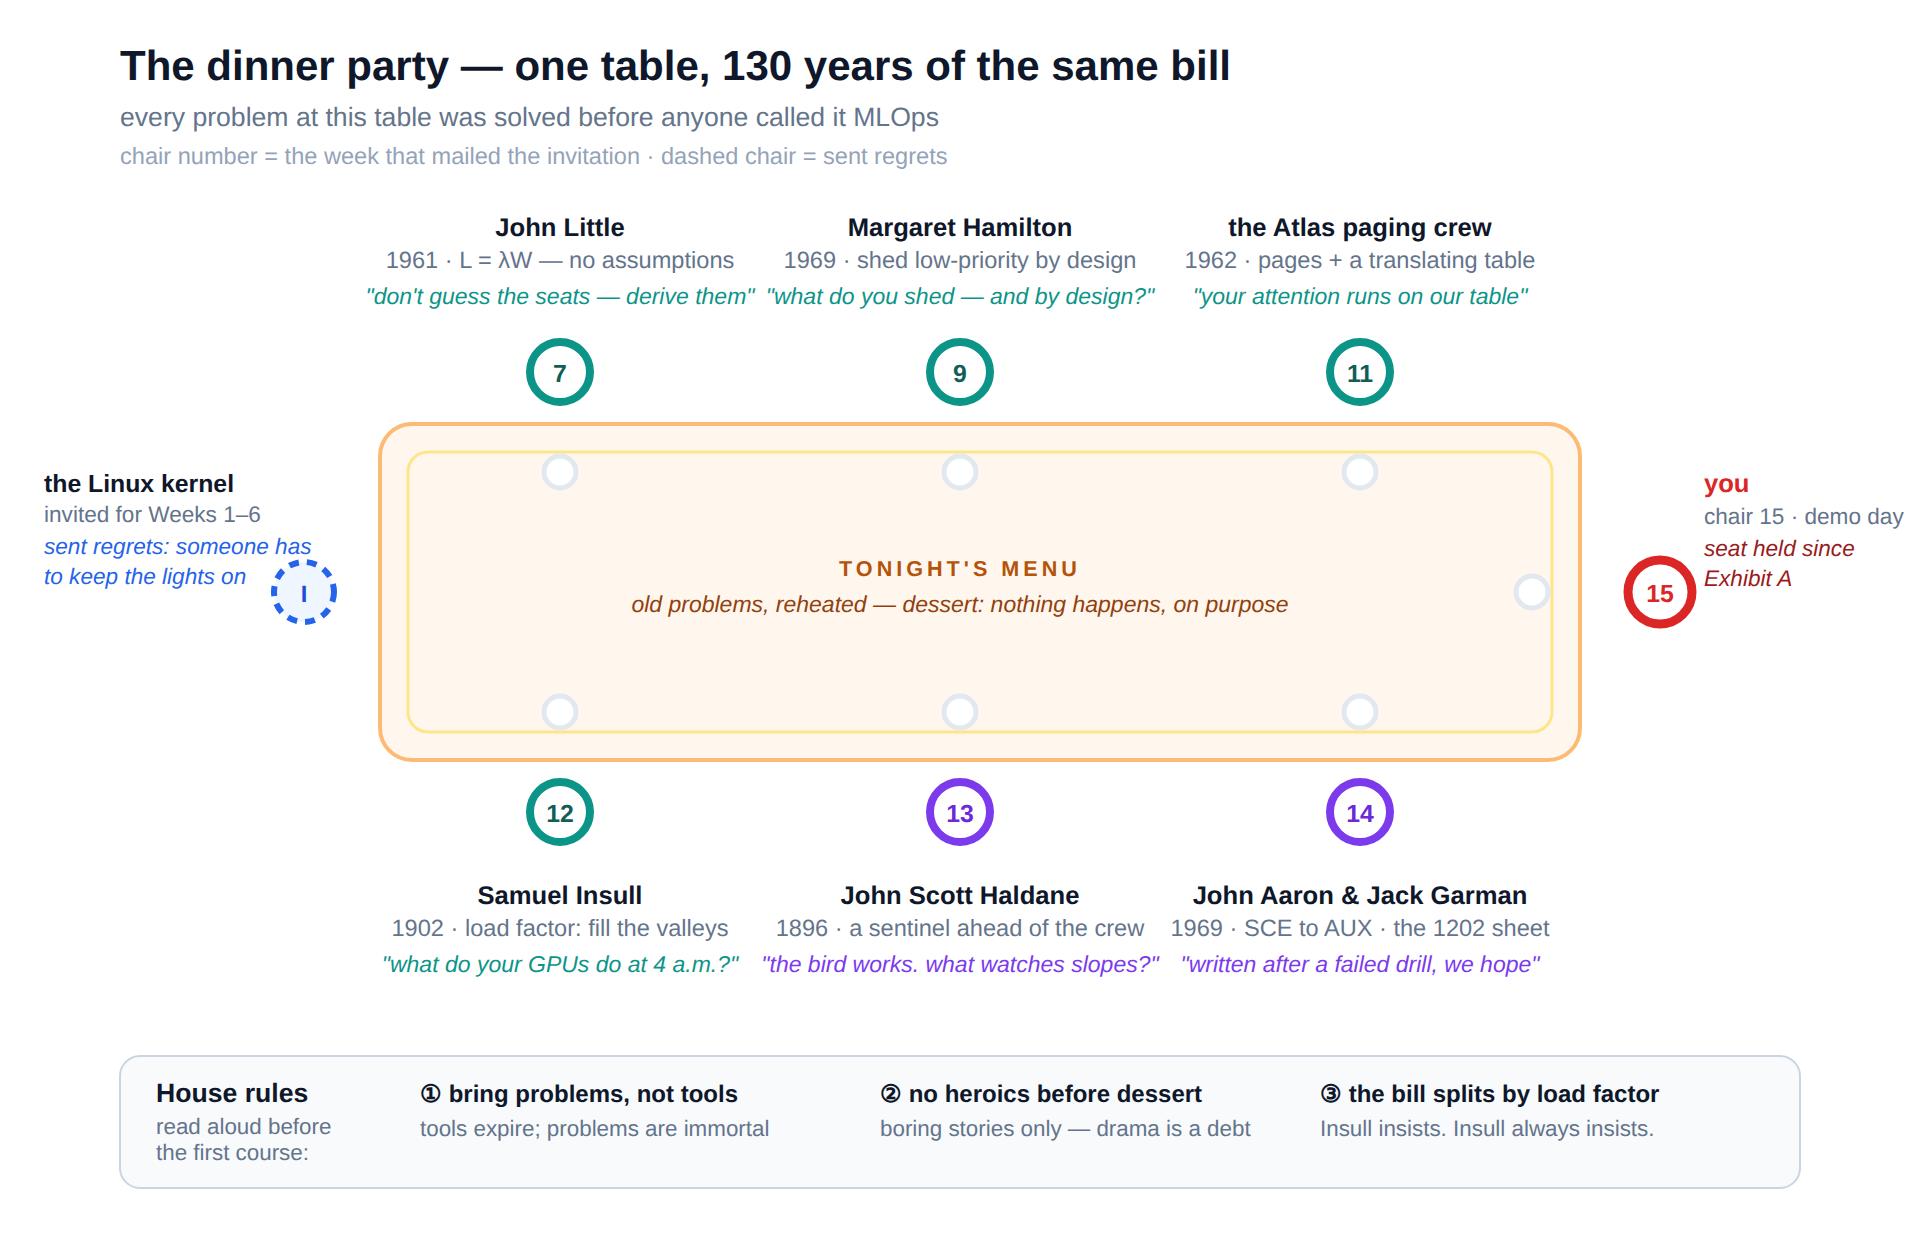
\includegraphics{figures/figE-2_dinner.png}}\\[3pt]
  \figcaption{Figure E-2  The seating chart. Chairs are numbered by the week that mailed the invitation; the kernel sent regrets; the seat at the head of the table is yours, and has been since Exhibit A. House rule three settles the bill.}
\end{tbbfigure}

\begin{calloutbox}{tbbteal}{tbbtealfill}
{\normalsize\bfseries\color{tbbteal}The point of the party}\par\vspace{3pt}
The party is a method, not a reward. The next impossible bill — energy, tokens, agents, whatever the 2030s put a meter on — will not be a new problem either, and the fastest engineer in the room will be the one who asks first: \textit{who paid this bill before computing existed, and what did they meter?} Steal older. The table adds a chair every decade or so, and the house style never changes: problems only. Tools are checked at the door, where they expire.
\end{calloutbox}

\vspace{4.0pt}

\namedsection{E.4}{The Warranty Card}

Every technical book ships with expiry dates; almost none print them. The reader finds out the hard way — quoting a retired flag in an interview, budgeting from a dead price sheet, losing an afternoon to a renamed YAML key — and concludes, wrongly, that the whole book spoiled. It did not. A systems book is mixed cargo: some of it is \textbf{milk}, some of it is \textbf{tinned goods}, and some of it is \textbf{cast iron}. The honest move is to label the crates. Here is the warranty card, printed in visible ink.

The dating test takes one second and works on any sentence in this book — or any other. Does the sentence contain a \textit{product name, a price, a version, or a ranking}? Milk: true in one lab, one region, one year; consume fresh and re-measure before you re-quote. Does it name an \textit{interface or a mechanism} — a digest, a cgroup file, a reconciliation loop, a histogram? Tinned: sealed against fashion for about a decade, because interfaces are treaties and treaties are expensive to break. Does it state an \textit{identity, a ratio, or a fact about humans under stress}? Cast iron. L = λW asked no favors of 1961 and asks none of you; load factor predates the vacuum tube; alarm fatigue has a body count. The iron tier survives a change of industry — which is the only durability test that means anything.

\begin{tbbtablewrap}
  \begin{tabular}{@{}>{\raggedright\arraybackslash}m{\dimexpr 0.3191\tbltextwidth-2\tabcolsep\relax} >{\raggedright\arraybackslash}m{\dimexpr 0.1596\tbltextwidth-2\tabcolsep\relax} >{\raggedright\arraybackslash}m{\dimexpr 0.5213\tbltextwidth-2\tabcolsep\relax}@{}}
  \arrayrulecolor{tbbnavy}\specialrule{1pt}{0pt}{0pt}
  \rowcolor{tbbtablehead}{\centering \bfseries\color{tbbnavy}Covered part} & {\centering \bfseries\color{tbbnavy}Class} & {\centering \bfseries\color{tbbnavy}Terms \& conditions} \\
  \arrayrulecolor{tbbnavy}\specialrule{0.7pt}{0pt}{2pt}
  \cellcolor{tbbxFFF7ED}{Names, prices, flags — vLLM switches, KEDA scalers, \$/GPU-hour, the \$4,762 → \$900 ledger, T4s and H100s, "small = 1–3 B", this season's quantization recipe} & \cellcolor{tbbxFFF7ED}{\centering \textcolor{tbbamberdark}{\textbf{Milk}\newline \textit{90 d – 3 yr}}} & \cellcolor{tbbxFFF7ED}{The numbers were true in one lab, one region, one year. What you actually bought is the \textit{method} that produced them — measure, gate, re-measure. Rerun it and get your own numbers; they will be better anyway.} \\
  \arrayrulecolor{tbbtableborder}\hline
  \cellcolor{tbbxFFF7ED}{League tables — Triton vs. TorchServe vs. BentoML vs. Ray Serve; what SageMaker and Vertex will and won't manage for you} & \cellcolor{tbbxFFF7ED}{\centering \textcolor{tbbamberdark}{\textbf{Milk}\newline \textit{90 d – 3 yr}}} & \cellcolor{tbbxFFF7ED}{Comparison tables spoil; the \textit{questions in their header rows} do not. Re-ask the same questions of whatever ships next, and accept different winners without grief.} \\
  \arrayrulecolor{tbbtableborder}\hline
  \cellcolor{tbbxEFF6FF}{Interfaces — OCI images and digests, cgroup v2 files, the reconciliation loop, Prometheus's series model, HTTP streams} & \cellcolor{tbbxEFF6FF}{\centering \textcolor{tbbnavy}{\textbf{Tinned}\newline \textit{≈ a decade}}} & \cellcolor{tbbxEFF6FF}{Treaties, not fashions. The dashboards above them get repainted yearly; underneath, a digest is still a hash, a limit is still a file the kernel reads, and desired state still converges. Learn once, carry between employers.} \\
  \arrayrulecolor{tbbtableborder}\hline
  \cellcolor{tbbxEFF6FF}{Mechanisms — continuous batching, paged KV, registry → gate → canary, autoscaling on two timescales, histograms for fleet percentiles} & \cellcolor{tbbxEFF6FF}{\centering \textcolor{tbbnavy}{\textbf{Tinned}\newline \textit{≈ a decade}}} & \cellcolor{tbbxEFF6FF}{These exist because of physics and people — weight streams, memory walls, diurnal humans — and neither is on a deprecation schedule. The names will churn and be acquired; the shapes will hold.} \\
  \arrayrulecolor{tbbtableborder}\hline
  \cellcolor{tbbxF0FDFA}{Arithmetic — L = λW; percentiles neither add nor average; the mean describes nobody; 128 + 9 = 137; load factor = average ÷ peak} & \cellcolor{tbbxF0FDFA}{\centering \textcolor{tbbteal}{\textbf{Cast iron}\newline \textit{10 yr, in writing}}} & \cellcolor{tbbxF0FDFA}{Little proved his law with no assumptions, which leaves nothing for time to break. Insull's ratio predates the vacuum tube. POSIX has promised you 137 for longer than the web has existed.} \\
  \arrayrulecolor{tbbtableborder}\hline
  \cellcolor{tbbxF0FDFA}{Ceremonies — the tolerance predates the number; page on symptoms, ticket on causes; blameless postmortems; boring = automated + versioned + gradual + reversible (+ observed)} & \cellcolor{tbbxF0FDFA}{\centering \textcolor{tbbteal}{\textbf{Cast iron}\newline \textit{10 yr, in writing}}} & \cellcolor{tbbxF0FDFA}{These regulate humans under stress, and humans are not receiving updates. The hospital data has a body count; the cheat sheet has a Moon landing. Valid for as long as 2 a.m. exists.} \\
  \arrayrulecolor{tbbtableborder}\hline
  \cellcolor{tbbxF0FDFA}{\textbf{The law — at 2 a.m. you can only see what you graphed at 2 p.m.}} & \cellcolor{tbbxF0FDFA}{\centering \textcolor{tbbteal}{\textbf{Cast iron}\newline \textit{lifetime}}} & \cellcolor{tbbxF0FDFA}{If this one ever fails, the failure will be visible only on a graph somebody drew in advance — which is the law winning again. Claims against this clause are usually called \textit{research results}.} \\
  \arrayrulecolor{tbbnavy}\specialrule{1pt}{2pt}{0pt}
  \end{tabular}\par
  \figcaption{The warranty card. Void where unmeasured.}
\end{tbbtablewrap}

\begin{calloutbox}{tbbamber}{tbbamberfill}
{\normalsize\bfseries\color{tbbamber}How to file a claim}\par\vspace{3pt}
Reproduce under load. Attach graphs drawn — per the terms above — in daylight. \textbf{Milk gone sour} is not a defect; check the date, rerun the benchmark, keep the method. \textbf{A tin failing inside its decade} entitles you to one indignant blog post and the industry's sincere apology. \textbf{Cast iron failing} — a queue that beats L = λW, a percentile that averaged honestly, a 2 a.m. debugged from pure memory — is not a warranty event at all: it is a publishable result, and the discipline pays those claims in citations. To date, none have been honored.
\end{calloutbox}

\vspace{4.0pt}

\namedsection{E.5}{A Letter for a Night That Hasn't Happened Yet}

One item remains, and it is sealed. Chapter 14 rehearsed a night with you — four dashboard rows, a burn rate, a neighbor on the GPU, twenty minutes, zero blame — but a rehearsal is a rehearsal, and somewhere ahead of you, an uncounted number of weeks from now, is the real thing: the first night a pager goes off and the service on the other end is \textit{yours}. No lab, no instructor, no answer key. This letter is for that night. Read it once now, so you know what it says; then put it wherever your future self keeps emergency supplies — taped into the runbook, pinned to the on-call handoff, folded behind the dashboard whose rows you will be reading when you remember it exists.

\begin{calloutbox}{tbbpurple}{tbbpurplefill}
{\normalsize\bfseries\color{tbbpurple}To be opened at 2:00 a.m.}\par\vspace{3pt}
Dear engineer —

If you are reading this on schedule, it is dark, something is wrong, and the pager chose you. Before you type anything: breathe once, on purpose. The service has already been broken for several minutes; it can spare you five more seconds. It survived its own death weekly in a lab. It was built to be exactly this hard to kill.

You have been here before, even though this night is new. Whatever is happening will feel unprecedented — they all do, at this hour — but it is almost certainly one of five old acquaintances: something \textbf{filled} (a queue, a disk, a pool of seats), something \textbf{was killed} (read the exit code; 137 means the meter was honest), something \textbf{changed} (find the deploy — and config counts; config \textit{always} counts), something \textbf{moved in} (a neighbor on your silicon, asking nothing, taking everything), or something \textbf{drifted} (the world, slowly, while the canary watched for cliffs). Five families. You have met every one of them in daylight, with coffee, in this book.

Read the rows in order; they were drawn for the brain you have right now, not the one you had at 2 p.m. The promise first: is the budget truly burning, or is this a cause dressed up as a symptom? Trust the burn rate over your adrenaline — both are measurements of the night, but only one of them is calibrated. If it is real, \textbf{mitigate before you understand}: the rollback is a pointer flip, it was rehearsed sober, and using it is not defeat — it is the design, working. A fast no beats a slow maybe, tonight most of all.

Type timestamps as you go — ugly, unpunctuated, straight into the channel; tomorrow-you will treat them as scripture. And keep tonight's job small: not truth — \textit{stability}. Truth is a daylight activity, performed blamelessly, in a document that names mechanisms and never people. Nobody serious will ask why you didn't see it sooner; the postmortem will simply add the panel that would have seen it — every fire leaves a smoke detector — and the next engineer's night will be twenty minutes shorter, the way one hand-written sheet of alarm codes once made a descent to the Moon thirty seconds calmer. Someone did this for you. Do it for the next one.

When it ends — and it will end sooner than it feels — notice what the ending is like: not triumphant. \textbf{Boring.} The graphs settle, the pager shrugs, the dashboard goes back to breathing. That is not anticlimax; that is the product. You spent fifteen weeks building not a service that cannot break — nobody has ever built one — but a night that ends early, a page that meant something, a fix that was a flip, and a morning whose only casualty is one alert threshold, adjusted.

Go back to bed. The service is fine. You made it boring — which was, from the first thirty seconds of silence, the entire point.

{\raggedleft \textcolor{tbbgray}{\textit{— written at 2 p.m., with the lights on}}\par}
\end{calloutbox}

\vspace{4.0pt}

That is the last exhibit. Fifteen weeks ago a perfect model sat behind thirty seconds of silence, and nobody in the room could say why. Tonight — some tonight — a boring service breathes on a dashboard, keeping a promise measured in milliseconds and a budget that ends in a chosen number, and nobody is watching, because nothing requires it. Between those two sentences sits everything this book had to say. Thank you for riding the Line 15 to the end of the line.

\begin{center}
{\large \textcolor{tbbink}{\textbf{Go build something boring.}}}
\end{center}

\begin{center}
\textcolor{tbbgray}{∎}
\end{center}
